\documentclass[12pt,letterpaper]{article}
\usepackage[utf8]{inputenc}
\usepackage[spanish]{babel}
\usepackage{graphicx}
\usepackage[left=2cm,right=2cm,top=2cm,bottom=2cm]{geometry}
\usepackage{graphicx} % figuras
% \usepackage{subfigure} % subfiguras
\usepackage{float} % para usar [H]
\usepackage{amsmath}
%\usepackage{txfonts}
\usepackage{stackrel} 
\usepackage{multirow}
\usepackage{enumerate} % enumerados
\renewcommand{\labelitemi}{$-$}
\renewcommand{\labelitemii}{$\cdot$}
% \author{}
% \title{Caratula}
\begin{document}

% Fancy Header and Footer
% \usepackage{fancyhdr}
% \pagestyle{fancy}
% \cfoot{}
% \rfoot{\thepage}
%

% \usepackage[hidelinks]{hyperref} % CREA HYPERVINCULOS EN INDICE

% \author{}
\title{Caratula}

\begin{titlepage}
\begin{center}
\large{UNIVERSIDAD PRIVADA-DE-TACNA}
\vspace*{-0.025in}
\begin{figure}[htb]
\begin{center}

\includegraphics[width=8cm]{./Imagenes/logo}
\end{center}
\end{figure}
\vspace*{0.15in}
INGENIERIA DE SISTEMAS  

\vspace*{0.5in}
\begin{large}
TITULO:\\
\end{large}

\vspace*{0.1in}
\begin{Large}
\textbf{INFORME DE LABORATORIO No 01} 
\end{Large}

\vspace*{0.3in}
\begin{Large}
\textbf{CURSO:} 
\end{Large}

\vspace*{0.1in}
\begin{large}
BASE DE DATOS II
\end{large}

\vspace*{0.3in}
\begin{Large}
\textbf{DOCENTE(ING):} 
\end{Large}

\vspace*{0.1in}
\begin{large}
 Patrick Cuadros Quiroga
\end{large}

\vspace*{0.2in}
\vspace*{0.1in}
\begin{large}
Integrantes: 
\begin{flushleft}
Orlando Antonio Acosta Ortiz		\hfill	(2015052775) \\
Orestes Ramirez Ticona              \hfill  (2015053236) \\
Nilson Laura Atencio     			\hfill 	(2015053846) \\
Roberto Zegarra Reyes 				\hfill 	(2010036175) \\
Richard Cruz Escalante 				\hfill 	(2013047247) \\
\end{flushleft}
\end{large}
\end{center}

\end{titlepage}


\tableofcontents % INDICE
\thispagestyle{empty} % INDICE SIN NUMERO
\newpage
\setcounter{page}{1} % REINICIAR CONTADOR DE PAGINAS DESPUES DEL INDICE

\section{Desarrollo de software basado en modelos (MBD)} 

\subsection{Proposito}
El propósito de esta técnica tiene los siguientes 3 objetivos básicos:

\subsection{El desarrollo de software basado en modelos (MBD)}
La ingeniería de software establece que el problema de construir software debe ser encarado de la misma forma en que los ingenieros construyen otros sistemas complejos, como puentes, edificios, barcos y aviones. La idea básica consiste en observar el sistema de software a construir como un producto complejo y a su proceso de construcción como un trabajo ingenieril. Es decir, un proceso planificado basado en metodologías formales apoyadas por el uso de herramientas. 
En los finales de los años 70 se observó un cambio importante en la filosofía del desarrollo de software, tendiente a solucionar los problemas descriptos arriba. Tom DeMarco en su libro Structured Analysis and System Specification [DeMarco 79] introdujo el concepto de ingeniería de software basada en modelos. DeMarco destacó que la construcción de un sistema de software debe ser precedida por la construcción de un modelo del sistema, tal como se realiza en otros sistemas ingenieriles. De esta forma, el modelo de un sistema provee un medio de comunicación y negociación entre usuarios, analistas y desarrolladores. Actualmente todos los métodos de desarrollo de software han adoptado esta filosofía. Lo que varía de un método a otro es la clase de modelos que deben construirse, la forma de representarlos, manipularlos, etc. El punto de partida en el proceso de desarrollo de software es la construcción de un modelo, el cual actúa como una especificación precisa de los requerimientos que el sistema debe satisfacer.  Un modelo del sistema consiste en una conceptualización del dominio del problema. El modelo  se focaliza sobre el mundo real: identificando, clasificando y abstrayendo los elementos que constituyen el problema y organizándolos en una estructura formal. 

\begin{center}
    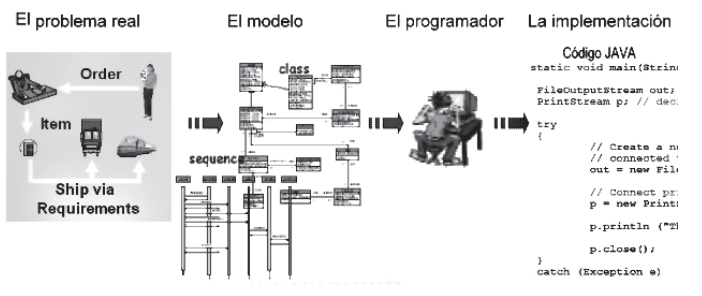
\includegraphics[width=12cm]{./Imagenes/mdd1}
    \end{center}

Actualmente casi todos los métodos de desarrollo de software utilizan modelos. Lo que varía de un método a otro es la clase de modelos que deben construirse, la forma de representarlos y manipularlos. A grandes rasgos podemos distinguir dos tendencias principales: los métodos matemáticos y los métodos diagramáticos.
Métodos Matemáticos:
Estos métodos utilizan lenguajes de especificación de naturaleza matemática, tales como: Z [DB 01], VDM [EF 94], B [BM 00] y OCL [OCL], los cuales permiten demostrar si la especificación cumple ciertas propiedades (ej., consistencia), derivar información implícita a partir de la especificación (ej., usando probadores de teoremas), derivar código automáticamente (ej., aplicando cálculos de refinamientos [BW 98]), verificar formalmente que el software satisface la especificación (ej., aplicando la lógica de Hoare [Hoare 69]).
Métodos Diagramáticos:
Por otra parte, los procesos basados en modelos gráficos –como el UP [JBR 99] con su especialización RUP (Rational Unified process) [Krutchten 00]– constituyen una propuesta más amigable, fácil de utilizar y comprender que los métodos formales. El éxito de estos procesos se basa principalmente en el uso de lenguajes diagramáticos, tales como UML [UML 03] que transmiten un significado intuitivo. A diferencia de las notaciones matemáticas, estos lenguajes diagramáticos son aceptados más fácilmente por los desarrolladores de software.

El ciclo de vida basado en modelos
El proceso de desarrollo de software, como se utiliza hoy en día, es conducido por el diseño de bajo nivel y por el código.
•	La conceptualización y la determinación de los requisitos del usuario 
•	Análisis y descripción funcional 
•	Diseño 
•	Codificación
•	Testeo 
•	Emplazamiento

\begin{center}
    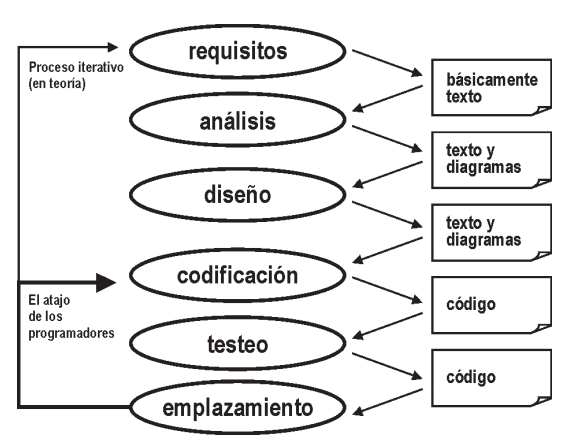
\includegraphics[width=12cm]{./Imagenes/mdd2}
    \end{center}

En las primeras fases se construyen distintos modelos tales como los modelos de los requisitos (generalmente escritos en lenguaje natural), los modelos de análisis y los modelos de diseño (frecuentemente expresados mediante diagramas). Estas fases pueden realizarse de una manera iterativa-incremental o en forma de cascada. En la práctica cotidiana, los modelos quedan rápidamente desactualizados debido al atajo que suelen tomar los desarrolladores en el ciclo de vida de este proceso.
Los problemas del desarrollo basado en modelos 
A continuación, analizamos algunos de los problemas más importantes encontrados durante el desarrollo de software basado en modelos y explicamos sus causas.
El problema de la productividad, el mantenimiento y la documentación: Muchas veces se considera la tarea de la documentación como una sobrecarga adicional. Se cree que escribir código es productivo, pero hacer modelos y documentación no lo es. Dada la complejidad de los sistemas de software actuales, resulta imprescindible contar con documentación en los distintos niveles de abstracción. Planteado así, quedan dos alternativas: o utilizamos nuestro tiempo en las primeras fases del desarrollo del software construyendo la documentación y diagramas de alto nivel y nos preocupamos por mantenerlos actualizados, o utilizamos nuestro tiempo en la fase de mantenimiento descubriendo lo que hace realmente el software.
El problema de la flexibilidad a los cambios tecnológicos: La industria del software tiene una característica especial que la diferencia de las otras industrias. Cada año (o en menos tiempo), aparecen nuevas tecnologías que rápidamente llegan a ser populares (a modo de ejemplo, se pueden listar Java, Linux, XML, HTML, UML, .NET, JSP, ASP, PHP, flash, servicios de Web, etc.). Y muchas compañías necesitan aplicar estas nuevas tecnologías por buenas razones: - Los clientes exigen esta nueva tecnología (por ejemplo, implementaciones para web). - Son la solución para algunos problemas reales (por ejemplo, XML para el problema de intercambio de datos). - La empresa que desarrolla la herramienta deja de dar soporte a las viejas tecnologías y se centra sólo en las nuevas (por ejemplo, el soporte para OMT fue reemplazado por soporte para UML).




\subsection{El desarrollo de software dirigido por modelos (MDD)}

El Desarrollo de Software Dirigido por Modelos MDD (por sus siglas en inglés: Model Driven software Development) se ha convertido en un nuevo paradigma de desarrollo software. MDD promete mejorar el proceso de construcción de software basándose en un proceso guiado por modelos y soportado por potentes herramientas.
Los modelos se van generando desde los más abstractos a los más concretos a través de pasos de transformación y/o refinamientos, hasta llegar al código aplicando una última transformación. La transformación entre modelos constituye el motor de MDD.
Los puntos claves de la iniciativa MDD fueron identificados en [Booch 04b] de la siguiente forma: 
1-	El uso de un mayor nivel de abstracción en la especificación tanto del problema a resolver como de la solución correspondiente, en relación con los métodos tradicionales de desarrollo de software. 
2-	El aumento de confianza en la automatización asistida por computadora para soportar el análisis, el diseño y la ejecución. 
3-	El uso de estándares industriales como medio para facilitar las comunicaciones, la interacción entre diferentes aplicaciones y productos, y la especialización tecnológica.

\begin{center}
    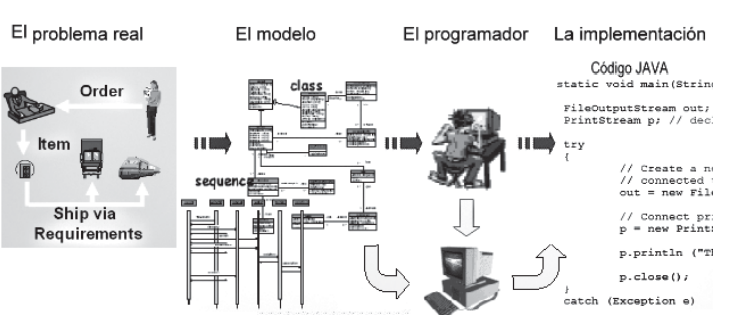
\includegraphics[width=12cm]{./Imagenes/mdd3}
    \end{center}

Abstracción: El enfoque de MDD para incrementar los niveles de abstracción es definir lenguajes de modelado específicos de dominio cuyos conceptos reflejen estrechamente los conceptos del dominio del problema, mientras se ocultan o minimizan los aspectos relacionados con las tecnologías de implementación.
Automatización: La automatización es el método más eficaz para aumentar la productividad y la calidad.
Estándares: MDD debe ser implementado mediante una serie de estándares industriales abiertos.
El ciclo de vida dirigido por modelos
Una de las mayores diferencias está en el tipo de los artefactos que se crean durante el proceso de desarrollo.
MDD identifica distintos tipos de modelos: - modelos con alto nivel de abstracción independientes de cualquier metodología computacional, llamados CIMs (Computational Independent Model), - modelos independientes de cualquier tecnología de implementación llamados PIMs (Platform Independent Model), - modelos que especifican el sistema en términos de construcciones de implementación disponibles en alguna tecnología específica, conocidos como PSMs (Platform Specific Model), - y finalmente modelos que representan el código fuente en sí mismo, identificados como IMs (Implementation Model).

\begin{center}
    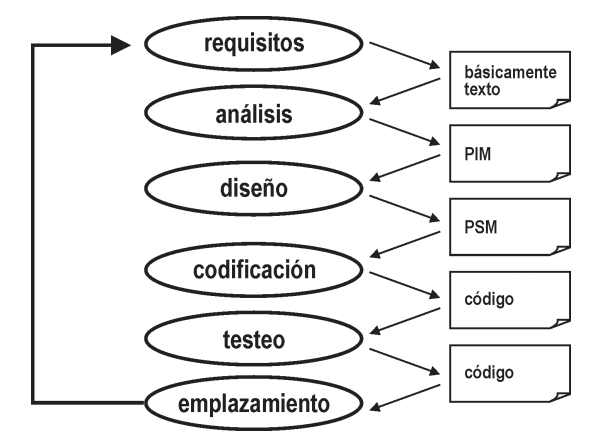
\includegraphics[width=12cm]{./Imagenes/mdd4}
    \end{center}

Muchas herramientas pueden transformar un PSM a código; no hay nada nuevo en eso. Dado que un PSM es un modelo muy cercano al código, esta transformación no es demasiado compleja. Lo novedoso que propone MDD es que las transformaciones entre modelos (por ejemplo de un PIM a PSMs) sean automatizadas.

\begin{center}
    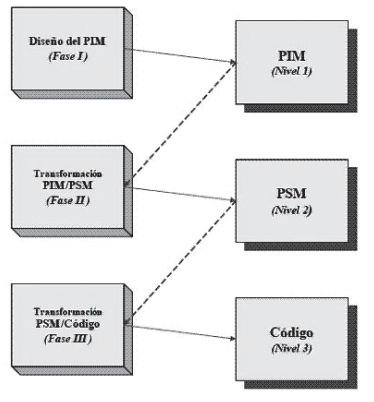
\includegraphics[width=12cm]{./Imagenes/mdd5}
    \end{center}

Orígenes de MDD
MDD es la evolución natural de la ingeniería de software basada en modelos enriquecida mediante el agregado de transformaciones automáticas entre modelos. Por su parte, la técnica de transformaciones sucesivas tampoco es algo novedoso. Podemos remitirnos al proceso de abstracción y refinamiento presentado por Edsger W. Dijkstra en su libro “A Discipline of Programming” [Dijkstra 76] donde se define que refinamiento es el proceso de desarrollar un diseño o implementación más detallado a partir de una especificación abstracta a través de una secuencia de pasos matemáticamente justificados que mantienen la corrección con respecto a la especificación original.
En general estas técnicas de refinamiento se limitan a transformar un modelo formal en otro modelo formal escrito en el mismo lenguaje (es decir, se modifica el nivel de abstracción del modelo, pero no su lenguaje), mientras que MDD es más amplio pues ofrece la posibilidad de transformar modelos escritos en distintos lenguajes (por ejemplo, podemos transformar un modelo escrito en UML en otro modelo escrito en notación Entidad-Relación).
Beneficios de MDD
Incremento en la productividad: MDD reduce los costos de desarrollo de software mediante la generación automática del código y otros artefactos a partir de los modelos, lo cual incrementa la productividad de los desarrolladores.
Adaptación a los cambios tecnológicos: el progreso de la tecnología hace que los componentes de software se vuelvan obsoletos rápidamente. MDD ayuda a solucionar este problema a través de una arquitectura fácil de mantener donde los cambios se implementan rápida y consistentemente, habilitando una migración eficiente de los componentes hacia las nuevas tecnologías.
Adaptación a los cambios en los requisitos: poder adaptarse a los cambios es un requerimiento clave para los negocios, y los sistemas informáticos deben ser capaces de soportarlos.
Consistencia: la aplicación manual de las prácticas de codificación y diseño es una tarea propensa a errores.
Re-uso: en MDD se invierte en el desarrollo de modelos y transformaciones.
Mejoras en la comunicación con los usuarios: los modelos omiten detalles de implementación que no son relevantes para entender el comportamiento lógico del sistema.
Mejoras en la comunicación entre los desarrolladores: los modelos facilitan el entendimiento del sistema por parte de los distintos desarrolladores.
Captura de la experiencia: las organizaciones y los proyectos frecuentemente dependen de expertos clave quienes toman las decisiones respecto al sistema.
Los modelos son productos de larga duración: en MDD los modelos son productos importantes que capturan lo que el sistema informático de la organización hace.
Posibilidad de demorar las decisiones tecnológicas: cuando aplicamos MDD, las primeras etapas del desarrollo se focalizan en las actividades de modelado.



\subsection{Propuestas Concretas para MDD}
Esto es realmente más técnica, porque con buenos hábitos de programación siempre se logra que el proyecto sea modular y reutilizable. Prepararlo para el cambio es una característica que no se consigue siempre y que con TDD si, ya que muchas veces cuando se tiene que cambiar la funcionalidad de la aplicación se tiene que refactorizar código ajeno, trabajar con código complicado, entre otras cosas; en cambio con TDD se tiene la confianza de que cuando se haga cambios no se van a estropear las funcionalidades que ya se tienen. Esto se consigue ya que la forma funcional de TDD es que primero se construye la prueba y luego el código hace que todo lo que surja en él ya este testeado, así que cualquier cambio que se vaya a introducir estará cubierto por los tests y si llegas a dañar algo alguno de ellos reaccionara cuando se ejecuten.
\textbf{}\\
Todo esto cambia un poco la mentalidad tradicional que es: primero analizar los requisitos, luego hacer un diseño completo y profesional, después empezar a codificar y por último testear. Lo que hay que hacer es que, en vez de planear tareas pensar en ejemplos y datos concretos, ya que en eso se basa los test, tener parámetros de entrada y de salida y luego ver si la respuesta es lo que se esperaba.
Si con TDD consigues tener en las especificaciones o requisitos una lista de ejemplos muy completa, que sean concretos, que elimine cualquier tipo de ambigüedad y que se puedan transformar en pruebas, al final tendrás una batería de tests que te cubrirán todas las funcionalidades y el código resultante estará 100\% cubierto por dichos test.

\section{Modelo Transformaciones y Herramientas}
\subsection{¿Qué es un modelo?}
El acrónimo MDD enfatiza el hecho de que los modelos son el foco central de MDD. Los modelos que nos interesan son aquellos relevantes para el desarrollo de software, sin embargo estos modelos no sólo representan al software; cuando un sistema de software soporta un determinado negocio, el modelo de dicho negocio es también relevante. Pero, ¿qué significa exactamente la palabra “modelo”? Necesitamos una definición que sea lo suficientemente general para abarcar varios tipos diferentes de modelos, pero que al mismo tiempo sea lo suficientemente específica para permitirnos definir transformaciones automáticas de un modelo a otro modelo. En el ámbito científico un modelo puede ser un objeto matemático (ej., un sistema de ecuaciones), un gráfico (ej., un plano) o un objeto físico (ej., una maqueta). El modelo es una representación conceptual o física a escala de un proceso o sistema, con el fin de analizar su naturaleza, desarrollar o comprobar hipótesis o supuestos y permitir una mejor comprensión del fenómeno real al cual el modelo representa y permitir así perfeccionar los diseños, antes de iniciar la construcción de las obras u objetos reales. Se utilizan con frecuencia para el estudio de represas, puentes, puertos, aeronaves, etc. Muchas veces, para obras complejas como por ejemplo una vivienda, se requiere la construcción de más de un modelo (figura 2-1). Por ejemplo, un modelo general de la disposición de los ambientes de la vivienda con sus puertas y ventanas, un modelo específico a una escala mayor para la instalación eléctrica y sanitaria, uno diferente para mostrar la estética de la fachada y el entorno, etc.
\\\\
\begin{figure}[H]
\centering
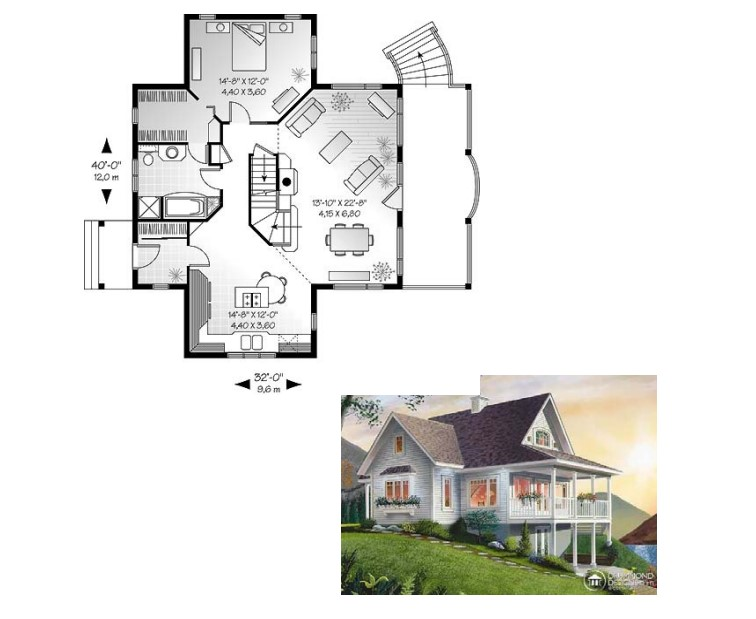
\includegraphics[scale=0.5]{./Imagenes/modelo1}
\caption{Ejemplo de figura 1-2}
\label{figura1}
\end{figure}

\subsection{Tipos de Modelos}
La definición de modelo dada en la sección anterior es muy amplia pues abarca muchos tipos diferentes de modelos. Los sistemas de software involucran varios modelos interdependientes a diferentes niveles de abstracción (análisis, diseño, implementación), representando diferentes partes del sistema (interfaz con el usuario, base de datos, lógica del negocio, administración del sistema), diferentes requisitos (seguridad, desempeño, flexibilidad), o diferentes tareas (modelos de pruebas, modelos de emplazamiento). En muchos casos, es posible generar un modelo a partir de otro, por ejemplo pasando del modelo de análisis al modelo de diseño, o del modelo de la aplicación al modelo de pruebas. Existen varias formas de distinguir entre tipos de modelos, cada una de ellas se basa en la respuesta a alguna pregunta acerca del modelo, por ejemplo:\\ \\
- ¿En qué parte del proceso de desarrollo de software es usado el modelo?\\
 - ¿El modelo es abstracto o es detallado?\\
 - ¿Qué sistema es descrito por el modelo? ¿Es un modelo del negocio o es un modelo de software?\\
 - ¿Qué aspectos del sistema son descritos por el modelo? ¿Es un modelo de la estructura o es un modelo del comportamiento?\\ 
- ¿Es un modelo orientado a una tecnología específica o es un modelo independiente de la tecnología?\\ \\
Las respuestas a estas preguntas nos permiten clasificar los diferentes tipos de modelos en categorías no disjuntas. En las siguientes secciones analizaremos en detalle esta clasificación.
\\\\

\subsection{Modelos a lo largo del proceso de desarrollo:}
Durante el proceso de desarrollo de software se crean diferentes modelos (figura 2-2). Los modelos de análisis capturan sólo los requisitos esenciales del sistema de software, describiendo lo que el sistema hará independientemente de cómo se implemente. Por otro lado, los modelos de diseño reflejan decisiones sobre el paradigma de desarrollo (orientado a objetos, basado en componentes, orientado a aspectos, etc.), la arquitectura del sistema (distintos estilos arquitecturales), la distribución de responsabilidades (GRASP patterns [Larman 04], GoF patterns [GHJV94]), etc. Finalmente, los modelos de implementación describen cómo el sistema será construido en el contexto de un ambiente de implementación determinado (plataforma, sistema operativo, bases de datos, lenguajes de programación, etc.). Si bien algunos modelos pueden clasificarse claramente como un modelo de análisis, o de diseño o de implementación, por ejemplo, un diagrama de casos de uso es un modelo de análisis, mientras que un diagrama de interacción entre objetos es un modelo de diseño y un diagrama de deployment es un modelo de implementación. En general, esta clasificación no depende del modelo en sí mismo sino de la interpretación que se de en un cierto proyecto a las etapas de análisis, diseño e implementación.
\begin{figure}[H]
\centering
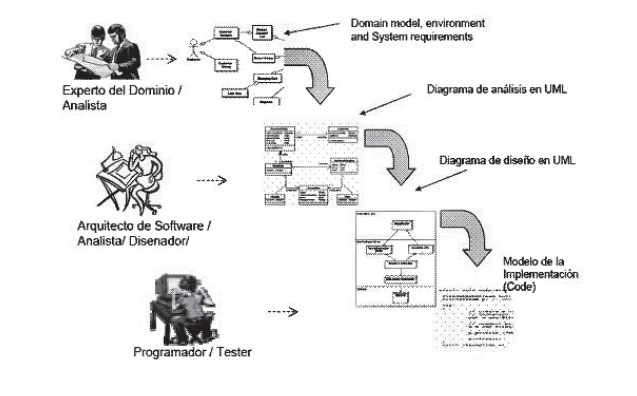
\includegraphics[scale=0.9]{./Imagenes/modelo2}
\caption{Ejemplo de figura 2}
\label{figura2}
\end{figure}

\subsection{Modelos abstractos y modelos detallados:}
 La clasificación entre modelo abstracto y modelo detallado también posee cierto grado de subjetividad. En general las herramientas de modelado nos permiten visualizar a un mismo modelo en distintos niveles de detalle [Egyed 02]. Por ejemplo podemos visualizar un diagrama de clases en forma abstracta limitando la información que se despliega sobre cada DESARROLLO DE SOFTWARE DIRIGIDO POR MODELOS clase sólo a su nombre, y limitando la profundidad de las jerarquías de herencia y composición a un máximo de k niveles. Luego podemos visualizar el diagrama en más detalle, incluyendo los nombres de los métodos públicos de cada clase y/o expandiendo las jerarquías de clases.
 
\subsection{Modelos de negocio y modelos de software:}
 Un modelo del negocio describe a un negocio o empresa (o parte de ellos). El lenguaje que se utiliza para construir el modelo del negocio contiene un vocabulario que permite al modelador especificar los procesos del negocio, los clientes, los departamentos, las dependencias entre procesos, etc. Un modelo del negocio no describe necesariamente detalles acerca del sistema de software que se usa en la empresa; por lo tanto a este modelo suele llamárselo “modelo independiente de la computación” (CIM). Cuando una parte del negocio es soportada por un sistema de software, se construye un modelo diferente para tal sistema. Este modelo de software es una descripción del sistema de software. El sistema de software y el sistema del negocio son conceptos diferentes en el mundo real, sin embargo los requisitos del sistema de software usualmente se derivan del modelo del negocio al cual el software brinda soporte. Para la mayoría de los negocios existen varios sistemas de software dándole soporte. Cada sistema de software se usa para asistir una parte del negocio. Por lo tanto, existe una relación entre un modelo del negocio y los diferentes modelos de software que describen al software que brinda soporte al negocio, como mostramos en la figura 2-3.
\begin{figure}[H]
\centering
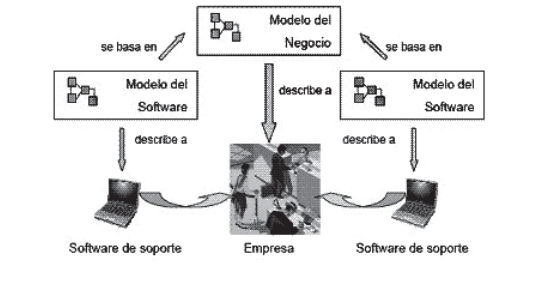
\includegraphics[scale=0.9]{./Imagenes/modelo3}
\caption{Ejemplo de figura 3}
\label{figura3}
\end{figure}

\subsection{Cualidades de los modelos:}
 El modelo de un problema es esencial para describir y entender el problema, independientemente de cualquier posible sistema informático que se use para su automatización. El modelo constituye la base fundamental de información sobre la que interactúan los expertos en el dominio del problema y los desarrolladores de software. Por lo tanto es de fundamental importancia que exprese la esencia del problema en forma clara y precisa. Por otra parte, la actividad de construcción del modelo es una parte crítica en el proceso de desarrollo. Los modelos son el resultado de una actividad compleja y creativa y por lo tanto son propensos a contener errores, omisiones e inconsistencias. La validación y verificación del modelo es muy importante, ya que la calidad del producto final dependerá fuertemente de la calidad de los modelos que se usaron para su desarrollo. Demos una mirada más detallada a las cualidades que esperamos encontrar en los modelos.\\\\ 
- Comprensibilidad. El modelo debe ser expresado en un lenguaje que resulte accesible (es decir entendible y manejable) para todos sus usuarios. \\\\
- Precisión. El modelo debe ser una fiel representación del objeto o sistema modelado. Para que esto sea posible, el lenguaje de modelado debe poseer una semántica precisa que permita la interpretación unívoca de los modelos. La falta de precisión semántica es un problema que no solamente atañe al lenguaje natural, sino que también abarca a algunos lenguajes gráficos de modelado que se utilizan actualmente.\\\\
- Consistencia. El modelo no debe contener información contradictoria. Dado que un sistema es representado a través de diferentes sub-modelos relacionados debería ser posible especificar precisamente cuál es la relación existente entre ellos, de manera que sea posible garantizar la consistencia del modelo como un todo. \\\\
- Completitud. El modelo debe capturar todos los requisitos necesarios. Dado que en general, no es posible lograr un modelo completo desde el inicio del proceso, es importante poder incrementar el modelo. Es decir, comenzar con un modelo incompleto y expandirlo a medida que se obtiene más información acerca del dominio del problema y/o de su solución.\\\\ 
- Flexibilidad. Debido a la naturaleza cambiante de los sistemas actuales, es necesario contar con modelos flexibles, es decir que puedan ser fácilmente adaptados para reflejar las modificaciones en el dominio del problema.\\\\
- Re-usabilidad. El modelo de un sistema, además de describir el problema, también debe proveer las bases para el re-uso de conceptos y construcciones que se presentan en forma recurrente en una amplia gama de problemas. \\\\
- Corrección. El análisis de la corrección del sistema de software debe realizarse en dos puntos. En primer lugar el modelo en sí debe ser analizado para asegurar que cumple con las expectativas del usuario. Este tipo de análisis generalmente se denomina ‘validación del modelo’. Luego, asumiendo que el modelo es correcto, puede usarse como referencia para analizar la corrección de la implementación del sistema Esto se conoce como ‘verificación del software’. Ambos tipos de análisis son necesarios para garantizar la corrección de un sistema de software.

\subsection{¿Qué es una transformación?}
 El proceso MDD, descrito anteriormente, muestra el rol de varios modelos, PIM, PSM y código dentro del framework MDD. Una herramienta que soporte MDD, toma un PIM como entrada y lo transforma en un PSM. La misma herramienta u otra, tomará el PSM y lo transformará a código. Estas transformaciones son esenciales en el proceso de desarrollo de MDD. En la figura 2-4 se muestra la herramienta de transformación como una caja negra, que toma un modelo de entrada y produce otro modelo como salida.
 
\begin{figure}[H]
\centering
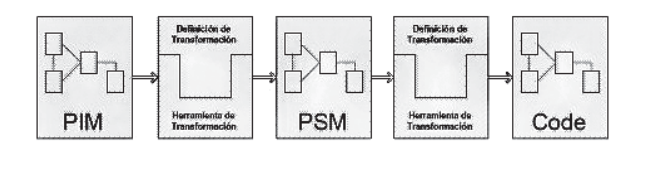
\includegraphics[scale=0.9]{./Imagenes/modelo4}
\caption{Ejemplo de figura 4}
\label{figura4}
\end{figure}

Si abriéramos la herramienta de transformación y mirásemos dentro, podríamos ver qué elementos están involucrados en la ejecución de la transformación. En algún lugar dentro de la herramienta hay una definición que describe como se debe transformar el modelo fuente para producir el modelo destino. Esta es la definición de la transformación. La figura 2-6 muestra la estructura de la herramienta de transformación. Notemos que hay una diferencia entre la transformación misma, que es el proceso de generar un nuevo modelo a partir de otro modelo, y la definición de la transformación. Para especificar la transformación, (que será aplicada muchas veces, independientemente del modelo fuente al que será aplicada) se relacionan construcciones de un lenguaje fuente en construcciones de un lenguaje destino. Se podría, por ejemplo, definir una transformación que relaciona elementos de UML a elementos Java, la cual describiría como los elementos Java pueden ser generados a partir de los elementos UML. Esta situación se muestra en la figura 2-5. DESARROLLO DE SOFTWARE DIRIGIDO POR MODELOS 53 En general, se puede decir que una definición de transformación consiste en una colección de reglas, las cuales son especificaciones no ambiguas de las formas en que un modelo (o parte de él) puede ser usado para crear otro modelo (o parte de él).\\

\begin{figure}[H]
\centering
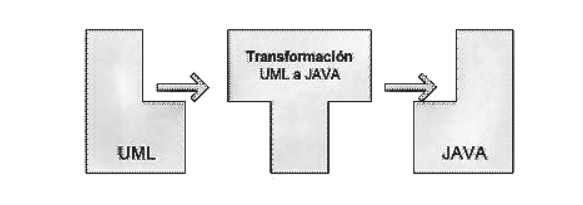
\includegraphics[scale=0.9]{./Imagenes/modelo5}
\caption{Ejemplo de figura 5}
\label{figura5}
\end{figure}

\subsection{¿Cómo se define una transformación?}
 Una transformación entre modelos puede verse como un programa de computadora que toma un modelo como entrada y produce un modelo como salida. Por lo tanto las transformaciones podrían describirse (es decir, implementarse) utilizando cualquier lenguaje de programación, por ejemplo Java. Sin embargo, para simplificar la tarea de codificar transformaciones se han desarrollado lenguajes de más alto nivel (o específicos del dominio de las transformaciones) para tal fin, tales como ATL [ATL] y QVT [QVT].
 
\subsection{Un ejemplo de transformación}
Exhibiremos un ejemplo de una transformación de un modelo PIM escrito en UML a un modelo de implementación escrito en Java. Transformaremos el diagrama de clases de un sistema de venta de libros (Bookstore) en las clases de Java correspondientes a ese modelo. La figura 2-8 muestra gráficamente la transformación que se intenta realizar, la cual consta de 2 pasos: Transformaremos el PIM en un PSM y luego transformaremos el PSM resultante a código Java

\begin{figure}[H]
\centering
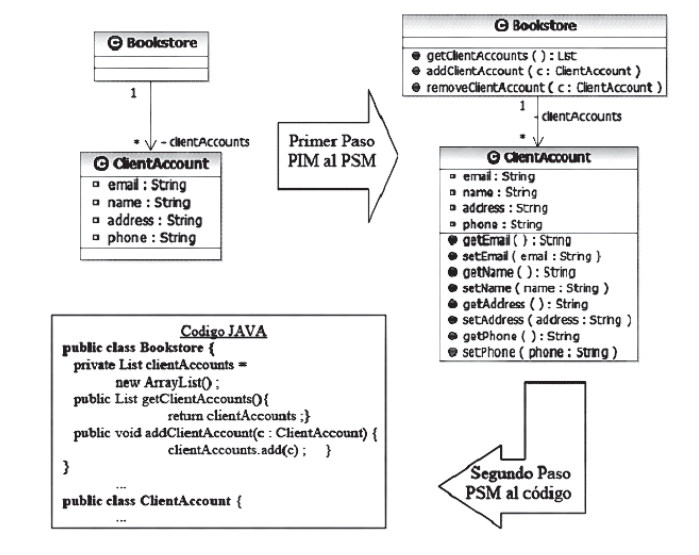
\includegraphics[scale=0.9]{./Imagenes/modelo6}
\caption{Ejemplo de figura 6}
\label{figura6}
\end{figure}

Tanto el PIM como el PSM son modelos útiles ya que proveen el nivel de información adecuado para diferentes tipos de desarrolladores y otras personas involucradas en el proceso de desarrollo de software. Existe una clara relación entre estos modelos. La definición de la transformación que debe aplicarse para obtener el PSM a partir del PIM consiste en un conjunto de reglas. Estas reglas son: \\\\
- Para cada clase en el PIM se genera una clase con el mismo nombre en el PSM. \\
- Para cada relación de composición entre una clase llamada classA y otra clase llamada classB, con multiplicidad 1 a n, se genera un atributo en la clase classA con nombre classB de tipo Collection. \\
- Para cada atributo público definido como attributeName:Type en el PIM los siguientes atributos y operaciones se generan como parte de la clase destino:\\ 
o Un atributo privado con el mismo nombre: attributeName: Type\\ 
o Una operación pública cuyo nombre consta del nombre del atributo\\ precedido con “get” y el tipo del atributo como tipo de retorno: getAttributeName(): Type \\
o Una operación pública cuyo nombre consta del nombre del atributo precedido con “set” y con el atributo como parámetro y sin valor de retorno: setAttributeName(att: Type). \\\\
El siguiente paso consistirá en escribir una transformación que tome como entrada el PSM y lo transforme a código Java. Combinando y automatizando ambas transformaciones podremos generar código Java a partir del PIM

\subsection{Herramientas de soporte para MDD}
 La puesta en práctica del proceso MDD requiere de la disponibilidad de herramientas de software que den soporte a la creación de modelos y transformaciones. La figura 2-9 brinda un panorama de los distintos puntos en los que el proceso MDD necesita ser soportado por herramientas. En particular, necesitamos los siguientes elementos:\\\\ 
- Editores gráficos para crear los modelos ya sea usando UML como otros lenguajes de modelado específicos de dominio.\\
- Repositorios para persistir los modelos y manejar sus modificaciones y versiones. \\
- Herramientas para validar los modelos (consistencia, completitud, etc.).\\
- Editores de transformaciones de modelos que den soporte a los distintos lenguajes de transformación, como QVT o ATL.\\
- Compiladores de transformaciones, debuggers de transformaciones.\\
- Herramientas para verificar y/o testear las transformaciones.

\begin{figure}[H]
\centering
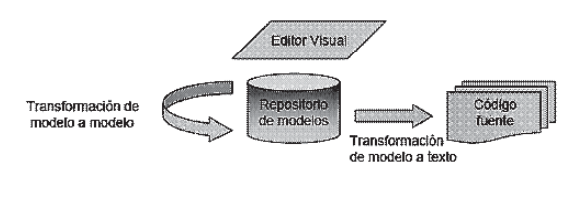
\includegraphics[scale=0.9]{./Imagenes/modelo7}
\caption{Ejemplo de figura 7}
\label{figura7}
\end{figure}




\section{Definicion formal de lenguajes de modelado.
El rol del metamodelo}
Aca se habla de los mecanismos para definir la sintaxis de los lenguajes con los cuales se crean los modelos de un sistema.
\\
- Tecnicas de metamodelado.
\\
- Arquitectura de cuatro capas de modelado definida por el OMG
\\
- ¿Porque el metamodelado es tan importante en el contexte de MDD?
\\
\subsection{Mecanismos para definir la sintaxis de un lenguaje de modelado}
Hace algunos años, la sintaxis de los lenguajes se definía casi exclusivamente
usando Backus Naur Form (BNF). Este formalismo es una meta
sintaxis usada para expresar gramáticas libres de contexto, es decir,
una manera formal de describir cuáles son las palabras básicas del lenguaje
y cuáles secuencias de palabras forman una expresión correcta
dentro del lenguaje.

Usando un lenguaje de modelado,
podemos crear modelos; un modelo especifica que elementos
pueden existir en un sistema. Si se define la clase Persona en un modelo,
se pueden tener instancias de Persona como Juan, Pedro, etc. Por otro
lado, la definición de un lenguaje de modelado establece que elementos
pueden existir en un modelo. Por ejemplo, el lenguaje UML establece que
dentro de un modelo se pueden usar los conceptos Clase, Atributo, Asociación,
Paquete, etc. Debido a esta similitud, se puede describir un lenguaje
por medio de un modelo, usualmente llamado “metamodelo”. El
metamodelo de un lenguaje describe que elementos pueden ser usados
en el lenguaje y como pueden ser conectados.
Como un metamodelo es también un modelo, el metamodelo en sí mismo
debe estar escrito en un lenguaje bien definido. Este lenguaje se
llama metalenguaje. Desde este punto de vista, BNF es un metalenguaje.
En la figura 3-1 se muestra gráficamente esta relación.

\begin{figure}[H]
\centering
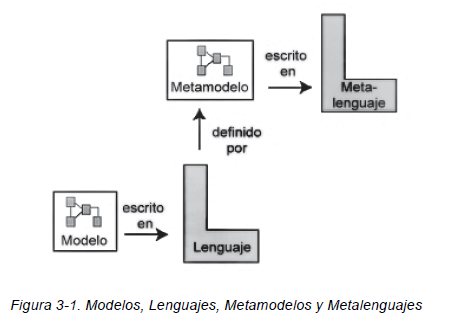
\includegraphics[scale=0.9]{./Imagenes/modelo8}
\end{figure}

\subsection{La arquitectura de 4 capas de modelado del OMG}

El metamodelado es entonces un mecanismo que permite definir formalmente
	lenguajes de modelado, como por ejemplo UML. La Arquitectura
	de cuatro capas de modelado es la propuesta del OMG orientada a
	estandarizar conceptos relacionados al modelado, desde los más abstractos
	a los más concretos.
\\
\\
\textbf{Nivel M0: Instancias}

En el nivel M0 se encuentran todas las instancias “reales” del sistema,
es decir, los objetos de la aplicación. Aquí no se habla de clases, ni
atributos, sino de entidades físicas que existen en el sistema.

\begin{figure}[H]
\centering
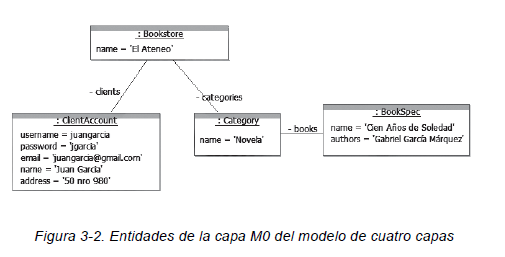
\includegraphics[scale=0.9]{./Imagenes/modelo9}
\end{figure}


\textbf{Nivel M1: Modelo del sistema}

Por encima de la capa M0 se sitúa la capa M1, que representa el modelo
de un sistema de software. Los conceptos del nivel M1 representan categorías
de las instancias de M0. Es decir, cada elemento de M0 es una
instancia de un elemento de M1. Sus elementos son modelos de los datos.

\begin{figure}[H]
\centering
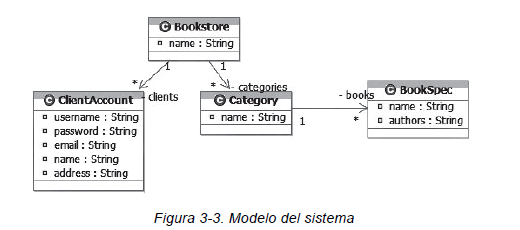
\includegraphics[scale=0.9]{./Imagenes/modelo10}
\end{figure}


\textbf{Nivel M2: Metamodelo}

Análogamente a lo que ocurre con las capas M0 y M1, los elementos del
nivel M1 son a su vez instancias del nivel M2. Esta capa recibe el nombre
de metamodelo.

\begin{figure}[H]
\centering
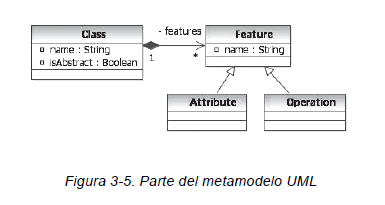
\includegraphics[scale=0.9]{./Imagenes/modelo11}
\end{figure}

Siguiendo el ejemplo, la entidad ClientAccount será una instancia de la
metaclase Class del metamodelo UML. Esta instancia tiene cinco objetos
relacionados a través de la meta asociación feature, por ejemplo una instancia
de Attribute con name=’username’ y type=’String’ y otra instancia
de Attribute con name=’password’ y type=’String’.
La figura 3-6 muestra la relación entre los elementos del nivel M1 con los
elementos del nivel M2.

\begin{figure}[H]
\centering
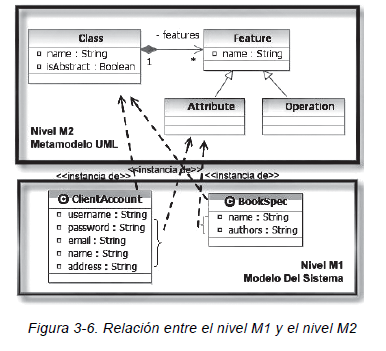
\includegraphics[scale=0.9]{./Imagenes/modelo12}
\end{figure}


\textbf{Nivel M3: Meta-metamodelo}

De la misma manera podemos ver los elementos de M2 como instancias de
otra capa, la capa M3 o capa de meta-metamodelo. Un meta-metamodelo es
un modelo que define el lenguaje para representar un metamodelo. La relación
entre un meta-metamodelo y un metamodelo es análoga a la relación
entre un metamodelo y un modelo.
M3 es el nivel más abstracto, que permite definir metamodelos concretos.
Dentro del OMG, MOF es el lenguaje estándar de la capa M3. Esto supone
que todos los metamodelos de la capa M2, son instancias de MOF.

\begin{figure}[H]
\centering
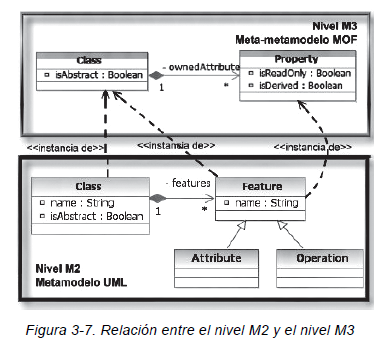
\includegraphics[scale=0.9]{./Imagenes/modelo13}
\end{figure}

\subsection{El uso del metamodelado en MDD}
Las razones por las que el metamodelado es tan importante en MDD son:

- En primer lugar, necesitamos contar con un mecanismo para definir lenguajes
de modelado sin ambigüedades [CESW 04] y permitir que una herramienta
de transformación pueda leer, escribir y entender los modelos.

- Luego, las reglas de transformación que constituyen una definición
de una transformación describen como un modelo en un lenguaje
fuente puede ser transformado a un modelo en un lenguaje destino.
Estas reglas usan los metamodelos de los lenguajes fuente y destino
para definir la transformación.

\begin{figure}[H]
\centering
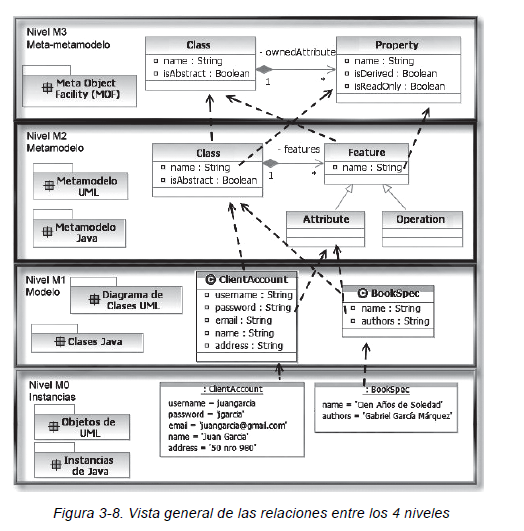
\includegraphics[scale=0.9]{./Imagenes/modelo14}
\end{figure}

- Y finalmente, la sintaxis de los lenguajes en los cuales se expresan
las reglas de transformación también debe estar formalmente definida
para permitir su automatización. En este caso también se utilizará
la técnica de metamodelado para especificar dicha sintaxis.

\begin{figure}[H]
\centering
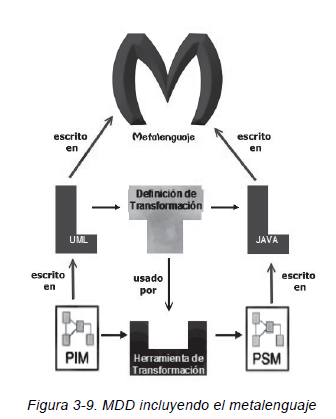
\includegraphics[scale=0.9]{./Imagenes/modelo15}
\end{figure}

\subsection{El lenguaje de modelado más abstracto: MOF}

El lenguaje MOF, acrónimo de Meta-Object Facility, es un estándar del
OMG para la ingeniería conducida por modelos. Como se vio anteriormente,
MOF se encuentra en la capa superior de la arquitectura de 4
capas. Provee un meta-meta lenguaje que permite definir metamodelos
en la capa M2. El ejemplo más popular de un elemento en la capa M2 es
el metamodelo UML, que describe al lenguaje UML.
Esta es una arquitectura de metamodelado cerrada y estricta.

\begin{figure}[H]
\centering
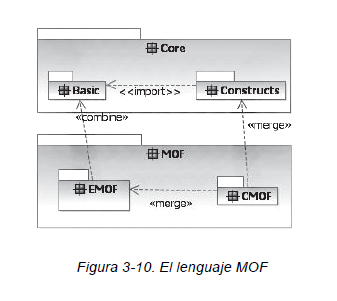
\includegraphics[scale=0.9]{./Imagenes/modelo16}
\end{figure}


\subsection{Ejemplos de metamodelos}

MOF puede ser usado para definir metamodelos de lenguajes orientados
a objetos, como es el caso de UML, y también para otros lenguajes
no orientados a objetos, como es el caso de las redes de Petri o los
lenguajes para servicios web.
En esta sección mostramos algunos ejemplos de metamodelos, en
particular la figura 3-12 muestra el metamodelo simplificado del lenguaje
UML donde se especifica que un modelo UML está formado por
paquetes (Package), donde cada paquete está integrado por clases
(Clase) que poseen atributos (Attribute). Los atributos tienen un nombre
(name) y un tipo (type), que puede ser un tipo de dato primitivo
(PrimitiveDataType) o una clase.

\begin{figure}[H]
\centering
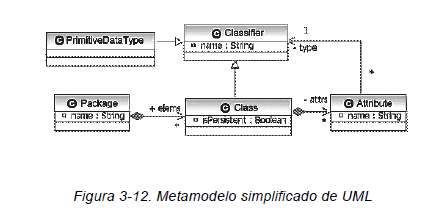
\includegraphics[scale=0.9]{./Imagenes/modelo17}
\end{figure}

El metamodelo del lenguaje RDBMS que mostramos en la figura 3-13
indica que un modelo relacional consta de esquemas (Schema), donde
cada esquema está compuesto por tablas (Table) que tienen columnas
(Column). Las columnas tienen un nombre (name) y un tipo de dato
(type). La tabla tiene una clave primaria (pkey) y cero o más claves
foráneas (fkeys). Cada clave foránea (Kkey) hace referencia a columnas
en otras tablas.

\begin{figure}[H]
\centering
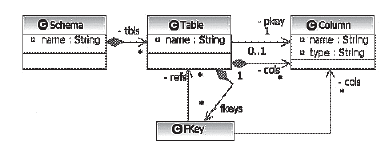
\includegraphics[scale=0.9]{./Imagenes/modelo18}
\end{figure}


\section{Herramientas de soporte a la creacion de modelos de software}

\begin{spacing}{4.0}
\end{spacing}
\subsection{Una arquitectura de dos niveles: modelo vs. metamodelos}
\begin{spacing}{2.0}
\end{spacing}
Los lenguajes de modelado visuales son lenguajes gráficos que se usan para la especificación,
visualización, documentación de productos de software como paso previo a su construcción.
Generalmente el marco conceptual de las notaciones de modelado se basa sobre una arquitectura
formada por distintos niveles (ver figura 5 [Odell95]). La descripción de esta arquitectura puede
encontrarse por ejemplo en [UML 97b].
\\\\
\begin{figure}[H]
\centering
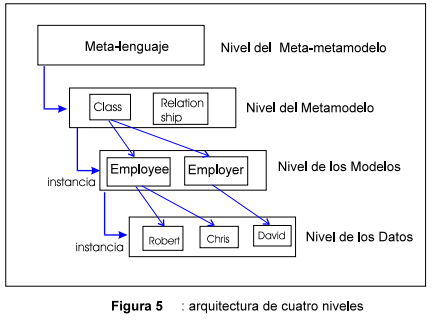
\includegraphics[scale=0.5]{./Imagenes/modelo19}
\caption{Ejemplo de figura 1-2}
\label{figura1}
\end{figure}
\subsection{Existen dos niveles principales:}
\begin{spacing}{2.0}
\end{spacing}
\textbf{1. El nivel del metamodelo:}
\begin{spacing}{2.0}
\end{spacing}
El metamodelo es un modelo para la información que puede ser
expresada durante la construcción del modelo de un sistema. Básicamente, define los
elementos de modelado tales como Class diagrams, State machines, Sequence diagrams
en el metamodelo de UML. Además define en que forma estos elementos se relacionan para
conformar el modelo de un sistema. El metamodelo es una descripción del lenguaje de
modelado en sí. Su semántica es el conjunto de todos los modelos bien formados. El
metamodelo es independiente de cualquier modelo en particular, él describe los elementos
del lenguaje y las restricciones que deben cumplir todos los modelos, por ejemplo: “dentro
de un Classifier los nombres de los atributos no se repiten”
\begin{spacing}{2.0}
\end{spacing}

\textbf{2. El nivel del modelo:}
\begin{spacing}{2.0}
\end{spacing}
Por otro lado, el modelo es una instancia del metamodelo. El modelo
(en realidad un modelo no es una unidad sino que es un conjunto de diversos modelos
relacionados, tal como fue explicado en la sección 1.3) describe los objetos inherentes al
dominio de la aplicación que está siendo modelada, por ejemplo: Employer, Employee,
BankAccount, Client, etc. e incluye restricciones que deben ser satisfechas por los objetos
del sistema, por ejemplo “no se permiten extracciones cuando el saldo de una cuenta es
menor que cero”
\begin{spacing}{2.0}
\end{spacing}
\subsection{Existen además otros dos niveles relacionados con los anteriores:}
\begin{spacing}{2.0}
\end{spacing}

\textbf{1. El nivel de los datos:}
\begin{spacing}{2.0}
\end{spacing}
 En el nivel de los datos, las entidades son instancias de las clases del
modelo, por ejemplo los objetos Robert y Chris son instancias de la Clase Employee.
\begin{spacing}{2.0}
\end{spacing}
\textbf{2. El nivel del meta-metamodelo:}
\begin{spacing}{2.0}
\end{spacing}
Es necesario contar con un nivel superior describiendo el
lenguaje utilizado para expresar el metamodelo. Este nivel superior es llamado metametamodelo. Por ejemplo en esta tesis utilizaremos Dynamic Logic como meta-lenguaje.

\subsection{Herramientas de metamodelado}
\begin{spacing}{2.0}
\end{spacing}
Herramientas de metamodelado. Son las herramientas básicas para diseñar el metamodelo de acuerdo al lenguaje de metamodelado, tal como se plantea en (Gómez y Sánchez, 2006).

\subsection{Ventajas}
\begin{spacing}{2.0}
\end{spacing}

Según (Quasar Tecnología, 2007) la aplicación de herramientas de metamodelado en una entidad o proyecto puede traer consigo varias ventajas, entre las que se encuentran

\begin{spacing}{2.0}
\end{spacing}

\begin{itemize}
    \item Reducción en tiempo y recursos para el mantenimiento de las aplicaciones existentes.

Todo desarrollador de software sabe que los productos que realizan, por representar modelos de lo que ocurre en el mundo real, son cambiantes y dinámicos, por lo que deben ser adaptables a las nuevas exigencias de los clientes o beneficiarios institucionales, esto conlleva a realizar un proceso que involucra grandes cambios. La aplicación del metamodelado, implica que los pasos a seguir para realizar la misma modificación sean menores. Este cambio en el paradigma del mantenimiento de las aplicaciones genera sustanciales beneficios a la organización que toma la decisión de adoptar esta tecnología para la construcción y mantenimiento de sus sistemas de información.

    \item Evita la introducción de errores en los programas.

La capacidad de introducir una nueva funcionalidad en un sistema de información sin escribir líneas de código adicional, elimina la posibilidad de introducir errores de programación cuyo costo tanto para la información registrada (errores en la base de datos a causa de un programa erróneo) o el costo de ubicar, corregir y probar el código fuente causante del error, son eliminados.

    \item Reducción en el tiempo de entrenamiento a los usuarios.

Luego de entrenar un usuario en la utilización de estas herramientas, el entrenamiento para que aprenda a utilizar la aplicación del metamodelo para otras aplicaciones, se reduce a trabajar con éste sobre los formatos, grupos y campos de información con los cuales se ha estructurado la información en el nuevo contexto. Esto gracias a la unicidad de las interfaces en el software de registro y consulta de información.

    \item Generación de consultas a la medida.

El sistema generador de consultas para un metamodelo, se convierte en una herramienta muy poderosa en manos de las personas que dominan el contexto temático de la información registrada en este metamodelo, ya que puede consultar, ordenar, agrupar, graficar o producir información alfanumérica para la información registrada

\end{itemize}

\subsection{AToM3}
\begin{spacing}{2.0}
\end{spacing}

A Tool for Multi-Formalism Modelling and Meta-Modelling (AToM3) es una herramienta MetaCASE escrita en el lenguaje de programación Python, y está enfocada a los flujos de trabajo de Análisis y Diseño. Posee un procesador que incluye un meta-metamodelo inicial basado en el modelo entidad-relación, que permite la definición de los diferentes metamodelos en un entorno gráfico con las mismas características que emplea el usuario en la construcción de los diferentes modelos. De esta manera, se puede definir cualquier tipo de metamodelo en términos de las entidades que forman parte del mismo y sus posibles interconexiones o relaciones. Una vez definido el metamodelo, se puede emplear su definición para construir los modelos pertinentes a un problema específico del mundo.(Zapata y Álvarez, 2005)

AToM3 tiene la posibilidad de expresar restricciones en términos de gramáticas de grafos incorporadas a su entorno. Las gramáticas de grafos tienen similitudes con las gramáticas basadas en texto en el sentido de que pueden ser usadas para describir las transformaciones a un grafo determinado; la diferencia radica en que las reglas de ese tipo de gramáticas se expresan de manera gráfica y no a modo de texto.

Las gramáticas de grafos se definen como un conjunto de reglas que poseen un lado izquierdo (LHS, por sus siglas en inglés, left-hand side) que contiene las precondiciones (expresadas de forma gráfica) que deben ser cumplidas para activar una determinada regla y un lado derecho (RHS, por sus siglas en inglés, right-hand side) que contiene el grafo que remplazará el que equivale al lado izquierdo de la regla.

Para las reglas expresadas de esta manera se deben definir condiciones y acciones para ejecutar cuando la regla se active. La gramática de grafos de AToM3 posee también un mecanismo que va reescribiendo el modelo a medida que las diferentes reglas se van activando hasta que no haya reglas que se puedan ejecutar. (Zapata y Álvarez, 2005)

\begin{spacing}{2.0}
\end{spacing}

\subsection{AndroMDA}
\begin{spacing}{2.0}
\end{spacing}

AndroMDA (pronunciado “Andrómeda”) es una herramienta de metamodelado escrita en el lenguaje Java bajo la licencia Berkeley Software Distribution (BSD), que está enfocada a todo el proceso de desarrollo de software. Es un programa informático de tipo framework. Se considera un motor de transformación de modelos en código fuente.

AndroMDA convierte modelos de algunas herramientas de modelado UML en componentes listos para su despliegue en un gran número de lenguajes entre los que se encuentran Java, PHP, .NET, HTML, sólo con utilizar los cartuchos adecuados.

Estos cartuchos dirigen el desarrollo de aplicaciones basadas en componentes y son fundamentales para el proceso de generación de código. La herramienta permite la creación de mecanismos para la construcción de nuevos cartuchos. (AndroMDA, 2006)

\begin{spacing}{2.0}
\end{spacing}

\

\section{Aplicando MDD al Desarrollo de un Sistema de Venta de Libros por Internet}

Mostraremos como el modelo PIM de ese sistema es automaticamente transformado en un PSM considerablemente complejo y luego veremos como finalmente se llega al codigo ejecutable. La complejidad del ejemplo es considerable, sin embargo nos enfocaremos solo en una parte reducida pero suficientemente completa como para apreciar los detalles del proceso. En las siguientes secciones introduciremos los requisitos del sistema que tomamos como ejemplo y describiremos los modelos y transformaciones involucrados en su desarrollo

\subsection{El Sistema de Venta de Libros por Internet}


Libros por Internet, al estilo Amazon, que permite vender y comprar libros a través de Internet. Hemos instalado el ejemplo completo en el sitio http://www.lifia.info.unlp.edu.ar/bookstore. Los requisitos generales del sistema son los siguientes: 
1. El bookstore será un sistema basado en la web para la venta de libros.
2. El bookstore tiene libros de los que se conoce el nombre, descripción, los autores, el precio. 
Los libros están organizados por categorías. Un ejemplo para categorías puede ser novelas, cuentos, historia. Un mismo libro puede tener varias versiones, algunas impresas y otras digitales. De los impresos se conoce el tamaño físico, la presentación, el stock y el peso para el envío. De los digitales su tamaño en bytes y el formato del archivo que lo contiene. La presentación impresa puede ser de tapa dura, edición de lujo, etc.
3. El usuario debe poder agregar libros en un carrito de compras online, previo a realizar la compra. Al momento de finalizar la compra, se generará una orden que incluye los ítems agregados al carrito de compras. Una vez confirmada la orden, se le enviará un mail al usuario informándole los datos de la misma. Similarmente, el usuario debe poder sacar ítems de su carrito o actualizar las cantidades de un ítem pedido. 
4. El usuario debe ser capaz de mantener una lista con los libros que desea comprar más tarde. 
5. El usuario debe poder cancelar órdenes antes de que hayan sido enviadas. 
6. El usuario debe poder pagar con tarjeta de crédito o transferencia bancaria. 
7. El usuario podría devolver libros que ha comprado. 
8. El usuario debe poder crear una cuenta, de forma tal que el sistema recuerde sus datos (nombre de usuario, nombre y apellido, dirección, email, detalles de su tarjeta de crédito) en el momento de registrarse
9. El usuario debe ser capaz de buscar libros usando distintos métodos de búsqueda –título, autor, palabra clave o categoría– y luego podrá ver los detalles  de los resultados de su búsqueda. 
10. El usuario debe poder escribir una opinión acerca de sus libros favoritos. Las opiniones aparecerán junto con los detalles del libro.


\subsection{5.2 Aplicando MDD}

Identificaremos las partes del proceso de desarrollo de software que tienen especial significado dentro del framework MDD. Para comenzar debemos identificar el modelo PIM de nuestro sistema y luego debemos identificar cuáles son los modelos PSM y el código que se espera como resultado del proceso de desarrollo. También es necesario que definamos cuáles son las transformaciones que usaremos para generar el PSM y el código a partir del modelo PIM
Entonces, necesitamos construir un sistema basado en la web que satisfaga los requisitos planteados.

\begin{figure}[H]
\centering
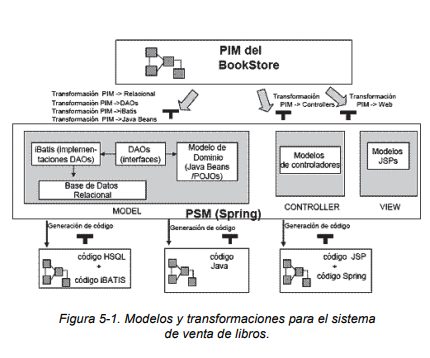
\includegraphics[scale=0.9]{./Imagenes/modelo20}
\caption{Ejemplo de figura 20}
\label{figura20}
\end{figure}


\subsection{5.2.1 El PIM y el PSM}

El primer paso en el proceso MDD consiste en la construcción de un modelo independiente de la plataforma (PIM) que describa (represente o modele) al sistema de venta de libros. Hemos elegido el lenguaje UML extendido mediante perfiles para expresar nuestro PIM. Se aplicaron los siguientes perfiles: MVC, Model, View y Session. En la figura 5-2 puede verse la definición de cada uno de ellos

\begin{figure}[H]
\centering
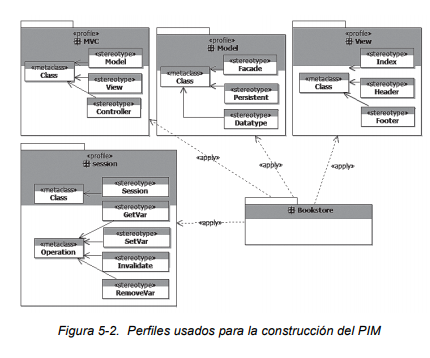
\includegraphics[scale=0.9]{./Imagenes/modelo21}
\caption{Ejemplo de figura 21}
\label{figura21}
\end{figure}

\subsection{5.2.2 La transformación de PIM a PSM }

El PSM tiene una arquitectura Model-View-Controller de tres capas, por lo tanto definiremos transformaciones separadas desde el PIM a cada parte del PSM.
Una transformación de PIM a la capa Model del MVC. La capa model a su vez está estructurada en distintos niveles, ya que distingue a los objetos del dominio en sí mismos (POJOs), a los mecanismos de acceso a los datos y a los mecanismos de persistencia de los datos (base de datos)

\subsection{5.2.3 La transformación de PSM a Código}

El siguiente paso consistirá en generar código ejecutable para cada PSM. Dado que en el framework MDD el código también es considerado un modelo, podemos hablar de modelos de código escritos en algún lenguaje de programación. Para el sistema de venta de libros por Internet tenemos varios modelos de código, escritos en HSQL, XML, Java y JSP. Por lo tanto necesitamos escribir al menos tres transformaciones de PSM a código: Una transformación de modelos relacionales a HSQL: una transformación que toma como entrada un modelo relacional y produce el script necesario para crear las tablas en HSQL..


\subsection{5.3 El PIM en detalle }

Las figuras 5-3, 5-4 y 5-5a-c muestran el PIM del Sistema de Venta de Libros por Internet. Como mencionamos anteriormente, el PIM es el modelo que requiere mayor intervención humana a través de un proceso creativo. Aquí asumimos que el PIM ya ha sido creado, ya sea mediante un proceso semi-automático basado en la aplicación de heurísticas y patrones o bien utilizando un proceso completamente manual. Los modelos que mostramos en esta sección son el resultado final de dicho proceso.
 

Si abriéramos la herramienta de transformación y mirásemos dentro, podríamos ver qué elementos están involucrados en la ejecución de la transformación. En algún lugar dentro de la herramienta hay una definición que describe como se debe transformar el modelo fuente para producir el modelo destino. Esta es la definición de la transformación. La figura 2-6 muestra la estructura de la herramienta de transformación. Notemos que hay una diferencia entre la transformación misma, que es el proceso de generar un nuevo modelo a partir de otro modelo, y la definición de la transformación. Para especificar la transformación, (que será aplicada muchas veces, independientemente del modelo fuente al que será aplicada) se relacionan construcciones de un lenguaje fuente en construcciones de un lenguaje destino. Se podría, por ejemplo, definir una transformación que relaciona elementos de UML a elementos Java, la cual describiría como los elementos Java pueden ser generados a partir de los elementos UML. Esta situación se muestra en la figura 2-5. DESARROLLO DE SOFTWARE DIRIGIDO POR MODELOS 53 En general, se puede decir que una definición de transformación consiste en una colección de reglas, las cuales son especificaciones no ambiguas de las formas en que un modelo (o parte de él) puede ser usado para crear otro modelo


\subsection{5.3.1 Modelo de casos de uso}

La figura 5-3 presenta el diagrama de casos de uso del sistema. No es el diagrama de casos de uso completo, ya que mostrarlo agregaría una complejidad innecesaria.

\begin{figure}[H]
\centering
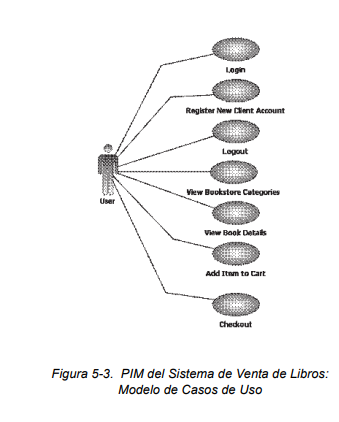
\includegraphics[scale=0.9]{./Imagenes/modelo22}
\caption{Ejemplo de figura 22}
\label{figura22}
\end{figure}


\subsection{5.3.2 Modelo estructural }

La figura 5-4 exhibe el diagrama de clases del sistema bookstore. Como puede verse en la figura, un bookstore tiene información acerca de sus clientes y de los libros que tiene en stock. Cada libro tiene una especificación de sus características y puede presentarse en dos versiones: digital o impreso. Los libros se organizan en categorías. Cada orden de compra está formada por varios ítems, donde se registra el ítem comprado, la cantidad y el precio pagado. Un usuario puede ir acumulando ítems en un carrito de compras y posteriormente efectivizar la compra de estos ítems. En la parte inferior de las figuras pueden verse definiciones escritas en OCL. Las primeras, por ejemplo, son las definiciones de dos operaciones en el contexto del carrito: getNumItems retorna la cantidad de elementos del carrito y getSubTotal retorna el total gastado.



\subsection{5.3.3 Modelos del comportamiento }

Para cada caso de uso se diseña un diagrama de secuencia mostrando la interacción de los elementos del sistema para llevar a cabo la funcionalidad pedida. Las figuras 5-5a-c muestran los diagramas que especifican el comportamiento del sistema bookstore para los casos de uso Login, Logout y View Book Details presentados anteriormente.

\begin{figure}[H]
\centering
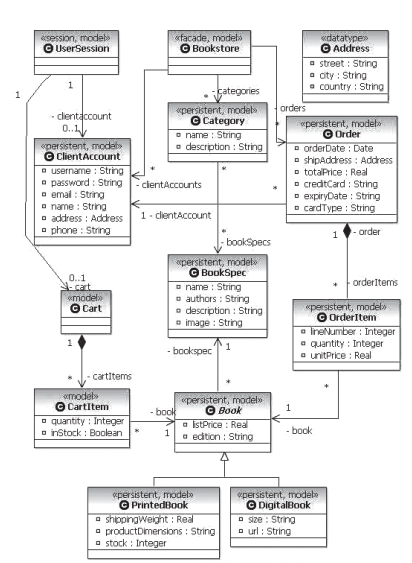
\includegraphics[scale=0.9]{./Imagenes/modelo23}
\caption{Ejemplo de figura 23}
\label{figura23}
\end{figure}

\include{Secciones/Actividad06}


\end{document}